% LAB 3: Functions
%
% CSE/IT 107: Introduction to Programming
% New Mexico Tech
%
% Prepared by Russell White and Christopher Koch
% Spring 2015

% - Functions
%   - Positional and Optional Arguments
%   - Recursion
% - Modules
%   - import statements
%   - main() boilerplate
% - Comments and PEP-8 style
% - Keywords: def
\documentclass[11pt]{cselabheader}
\fancyhead[R]{Lab 3: Functions}
\title{Lab 3: Functions}

\begin{document}
\pagenumbering{roman}
\maketitle

\begin{figure}[H]
  \centering
  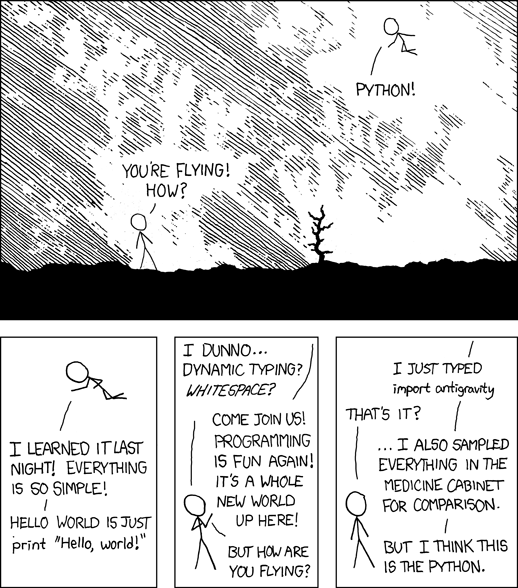
\includegraphics[width=0.85\textwidth]{img/xkcd_python.png}
  \caption{xkcd 353: Python (Source: \url{http://xkcd.com/353})}
\end{figure}

\pagebreak
\hrule
\begin{quotation}
``If you don't think carefully, you might believe that programming is just
typing statements in a programming language.''
\end{quotation}
\begin{flushright}
  --- W. Cunningham
\end{flushright}

\begin{quotation}
``Only ugly languages become popular. Python is the exception.''
\end{quotation}
\begin{flushright}
  --- Donald Knuth
\end{flushright}

\begin{quotation}
``The time you enjoy wasting is not wasted time.''
\end{quotation}
\begin{flushright}
  --- Bertrand Russell
\end{flushright}
\hrule

\tableofcontents

\pagebreak
\pagenumbering{arabic}

\section{Introduction}
\label{sec:intro}

In the previous lab, we showed you simple control flow and how to repeat a piece
of code using \pythoninline{while}. In this lab, we will be learning how to
break a lot of code into smaller, reusable pieces called \emph{functions}.

\section{Making Calculations Shorter}
\label{sec:calc}

We showed you simple Python operators such as \pythoninline{+},
\pythoninline{-}, \pythoninline{*}, \pythoninline{%},
etc in lab 1. There is a small extension to these that you can use to update a
variable:

\begin{pyconcode}
>>> x = 5
>>> x += 3 # same as x = x + 3
>>> x
8
\end{pyconcode}

The available assignment operators are:
\begin{multicols}{2}
\begin{itemize}
  \item \pythoninline{+=} -- addition
  \item \pythoninline{-=} -- subtraction
  \item \pythoninline{*=} -- multiplication
  \item \pythoninline{/=} -- division
  \item \pythoninline{//=} -- integer division
  \item \pythoninline{%=} -- remainder
  \item \pythoninline{**=} -- exponentiation
\end{itemize}
\end{multicols}
They each correspond to the non-assignment version.

\pagebreak
\section{Functions}
\label{sec:funcs}

We have used 

\subsection{Summary}
\label{subsec:funcs.sum}

\begin{itemize}
  \item A good resource:

\begin{center}
  \url{https://docs.python.org/3.4/tutorial/controlflow.html#defining-functions}
\end{center}

\end{itemize}

\subsection{Exercises}
\label{subsec:funcs.ex}

\pagebreak
\section{Conventions}
\label{sec:pep8}

In order to make code more readable, we will start requiring you to comment your
code and follow a style guide. Style guides are often used to make code easy to
read, especially if multiple people are working on a project together. If left
to their own devices, most people start conforming to their own style guide
anyway just by preferring a certain way to write something over another. For
example, common parameter of style guides is the use of a certain number of
spaces for indentation. Also, some people put spaces before each colon, and some
people do not.

\subsection{Style Guide}

We will be using PEP 8 (Python Enhancement Proposal 8 -- Style Guide for Python
Code) found at
\begin{center}
  \url{https://www.python.org/dev/peps/pep-0008/}
\end{center}

Some of the highlights:
\begin{itemize}
  \item 4 space indentation
  \item Function names should be all-lowercase with words separated by underscores.
  \item File/module/package names should have short, all-lowercase names.
  \item Comment your code with useful information. For example,

    \begin{python3code}
x = x + 1 # Increment x
    \end{python3code}

    should be avoided. It is obvious that \pythoninline{x} is being incremented.
    Instead, if you think a comment will improve code comprehension, the
    following can be useful:

    \begin{python3code}
x = x + 1 # Compensate for border
    \end{python3code}

  \item Avoid whitespace where it does not help code legibility. Never put a
    space between a function name and the parentheses when calling a function.

    \begin{python3code}
if x == 4: # do this
    print(x, y)

if x == 4 : # don't do this
    print ( x , y )
    \end{python3code}
\end{itemize}

\pagebreak
\subsection{Commenting Functions}

For commenting on functions, we will be using PEP 257 (Docstring Conventions)
found at
\begin{center}
  \url{https://www.python.org/dev/peps/pep-0257/}
\end{center}

\begin{center}
\bfseries \large You will be required to put a \emph{docstring} at the beginning
of every function that you code from now on.
\end{center}
A docstring is a comment immediately
following the function definition enclosed by triple-double-quotes (\texttt{"""}).

The highlights:
\begin{itemize}
  \item For short functions, do this:

    \begin{python3code}
def midpoint(a, b):
    """Find and return the midpoint of the given a and b."""
    return (a+b)/2
    \end{python3code}

  \item For larger functions or for a longer explanation, follow this style:

    \begin{python3code}
def calculate_weekly_pay(pay_rate, hours, tax_rate):
    """Calculate the net pay after taxes given the number of hours worked 
    in a week, a pay rate, and a flat tax rate.

    Arguments:
    pay_rate -- rate of pay
    hours -- number of hours worked in one week
    tax_rate -- flat tax rate (for example, 0.15 for 15%)
    """
    pay_before_taxes = hours * pay_rate

    # Add overtime payment if necessary
    if hours > 40:
        pay_before_taxes += (hours - 40) * pay_rate * 0.5

    pay_after_taxes = pay_before_taxes * (1 - tax_rate)
    return pay_after_taxes
    \end{python3code}

\end{itemize}

\pagebreak
\section{Modules}
\label{sec:modules}

A program that is saved in a text file and then run with Python is called a
\emph{script}. As your programs get longer, you may want to split them into
multiple files for easier legibility, maintenance, or abstraction. To do this,
Python supports a way to put definitions (of functions) in a file and use them
in another script or in the interpreter. A file like this is called a
\emph{module}. An example for such a module is the math module we have used
previously. The definitions from a module can be \emph{imported} into other
scripts.

A module is just a file with Python statements in it. A module takes the name of
the file that it is in. For example, imagine we have a file
\texttt{circlemath.py} in our current working directory:

\begin{python3code}
import math # importing the math module

def area(radius):
    """Find and return the area of a circle (float) given the radius"""
    return math.pi * radius**2

def circumference(radius):
    """Find and return the circumference of a circle (float) given the radius"""
    return 2 * math.pi * radius
\end{python3code}

Then, open the interpreter and import the module:

\begin{pyconcode}
>>> import circlemath
>>> circlemath.circumference(5) # have to use modulename.attributename
31.41592653589793
>>> circlemath.area(5)
78.53981633974483
>>> circlemath.__name__
'circlemath'
\end{pyconcode}

Every module has a \pythoninline{__name__} attribute that contains the name of
the module, except in one special case that we will see soon.

There are other kinds of import statements with different effects:

\begin{pyconcode}
>>> from circlemath import area
>>> area(5) # can just use the attribute imported without modulename.
78.53981633974483
>>> circumference(5) # not defined, because not imported
Traceback (most recent call last):
  File "<input>", line 1, in <module>
NameError: name 'circumference' is not defined
\end{pyconcode}

\begin{pyconcode}
>>> from circlemath import area, circumference # use commas to separate multiple
>>> area(5)
78.53981633974483
>>> circumference(5)
31.41592653589793
\end{pyconcode}

\begin{pyconcode}
>>> from circlemath import * # import all definitions made
>>> area(5)
78.53981633974483
>>> circumference(5)
31.41592653589793
\end{pyconcode}

\begin{pyconcode}
>>> from circlemath import area as carea
>>> carea(5)
78.53981633974483
\end{pyconcode}

The last option is rather frowned upon; we would prefer you to use
\pythoninline{circlemath.area} instead as it is more descriptive.

You may also rename a module upon importing it:

\begin{pyconcode}
>>> import circlemath as cmath
>>> cmath.area(5)
78.53981633974483
\end{pyconcode}


\begin{infobox}{Convention (PEP 8)}
  Always put \pythoninline{import} statements at the beginning of a file in the
  following order:
  \begin{enumerate}
    \item Built-in standard library modules
    \item Third-party modules (e.g. matplotlib)
    \item Self-written modules
  \end{enumerate}
  Put a blank line between each group of imports.
\end{infobox}

\subsection{Using Modules as Scripts and Boilerplate}

If there is code in your module that is not a function definition, Python will
run it just once when the module is imported. For example, take the file
\texttt{mid.py}:

\begin{python3code}
def midpoint(a, b):
    """Find and return the midpoint of two numbers."""
    return (a+b)/2

print('Midpoint of {} and {} is {:.2f}.'.format(5, 10, midpoint(5, 10)))
\end{python3code}

\begin{pyconcode}
>>> import mid
Midpoint of 5 and 10 is 7.50.
\end{pyconcode}

The same will happen if you run the module like a script:

\begin{bashcode}
$ python3 mid.py
Midpoint of 5 and 10 is 7.50.
\end{bashcode}

However, this can be rather annoying to deal with, for example if you wrote a
script with a bunch of functions a while ago and you just want to use the
functions you wrote, but do not want the other code to run when you're using
them -- you just want the functions. You can achieve this!

When you run a module as a script, the modules \pythoninline{__name__} attribute
is not set to the module's name, but to \pythoninline{"__main__"}. Hence, the
following code in \texttt{mid.py} will do the following:

\begin{python3code}
def midpoint(a, b):
    """Find and return the midpoint of two numbers."""
    return (a+b)/2

print(__name__) # just for demonstration, do not put this in real programs

if __name__ == "__main__":
    print('Midpoint of {} and {} is {:.2f}.'.format(5, 10, midpoint(5, 10)))
\end{python3code}

\begin{pyconcode}
>>> import mid
mid
\end{pyconcode}

\begin{bashcode}
$ python3 mid.py
__main__
Midpoint of 5 and 10 is 7.50.
\end{bashcode}

We call this specific if-statement referencing the \pythoninline{__name__}
variable boilerplate code.

\begin{infobox}{Boilerplate Requirement}
  Please put \textbf{any} code that is not part of a function inside the
  boilerplate if-statement so that \emph{every} one of your scripts can also be
  used as a module. This will be required for every lab from now on.

  Wrong:

  \begin{python3code}
print("Hello World!")
  \end{python3code}

  Right:

  \begin{python3code}
if __name__ == "__main__":
    print("Hello World!")
  \end{python3code}
\end{infobox}

\subsection{The \protect\pythoninline{dir()} Function}

Use the \pythoninline{dir()} function to get a list of every attribute --
variables, functions, and other things you do not know about yet -- that is part
of a module. For example for the circlemath module we wrote earlier:

\begin{pyconcode}
>>> import circlemath
>>> dir(circlemath)
['__name__', 'area', 'circumference']
>>> import mid
>>> dir(mid)
['__name__', 'midpoint']
>>> dir(math)
['__doc__', '__file__', '__loader__', '__name__', '__package__', '__spec__', 'acos',
'acosh', 'asin', 'asinh', 'atan', 'atan2', 'atanh', 'ceil', 'copysign', 'cos', 'cosh',
'degrees', 'e', 'erf', 'erfc', 'exp', 'expm1', 'fabs', 'factorial', 'floor', 'fmod',
'frexp', 'fsum', 'gamma', 'hypot', 'isfinite', 'isinf', 'isnan', 'ldexp', 'lgamma',
'log', 'log10', 'log1p', 'log2', 'modf', 'pi', 'pow', 'radians', 'sin', 'sinh', 'sqrt',
'tan', 'tanh', 'trunc']
\end{pyconcode}

\subsection{Summary}
\label{subsec:modules.sum}

\begin{itemize}
  \item Syntax:

    \begin{python3code}
import modname1, modname2 # use: modname1.attributename
import modname3 as othermodname # use: othermodname.attributename
from modname import attribute1, attribute2 # use: attribute1, attribute2
from modname import * # use: attributename
from modname import attribute as otherattribute # use: otherattribute
    \end{python3code}

    Attributes can be functions defined in the module or variables defined in
    the module. A special attribute is \pythoninline{__name__}, which contains
    the name of the module unless the module is executed as a script.

  \item Every script is a module whose name is the filename of the script.

  \item If a module is imported, its \pythoninline{__name__} attribute is a
    variable that contains the module name. If a module is run as a script, its
    \pythoninline{__name__} attribute contains \pythoninline{"__main__"}. With
    this, you can have code that only runs if a module is run like a script.

    We call that boilerplate code:

    \begin{python3code}
if __name__ == "__main__":
    # stuff that only runs if module is run as a script
    \end{python3code}

  \item Use \pythoninline{dir()} to get a list of every attribute -- every
    variable and function (and other things that you do not know about yet) --
    that is part of a particular module.

  \item A good resource:

    \begin{center}
\url{https://docs.python.org/3.4/tutorial/modules.html}
    \end{center}
\end{itemize}

\subsection{Exercises}
\label{subsec:modules.ex}

\pagebreak
\section{Advanced Functions}
\label{sec:adv}

\subsection{Positional and Optional Arguments}
\label{subsec:adv.args}

\subsection{Recursion}
\label{subsec:adv.recursion}

\subsection{Summary}
\label{subsec:adv.sum}

\subsection{Exercises}
\label{subsec:adv.ex}

\pagebreak
\section{Submitting}

Files to submit:
\begin{itemize}
  \item 
\end{itemize}

You should submit your code as a tarball. It should contain all files
used in the exercises for this lab. The submitted file should be named
\begin{center}
  \texttt{cse107\_firstname\_lastname\_lab3.tar.gz}
\end{center}

\begin{center}
  \textbf{Upload your tarball to Canvas before the deadline.}
\end{center}


\end{document}
